This section presents the results of the tests conducted on the simulated data. The tests include the marginal model test, the neural copula test, and the portfolio test, defined in \Cref{sec:Method}.

\subsection{Marginal Model Test}
The losses of the models in the marginal model test after training is shown in \Cref{tab:MarginalFinalLosses}. The table shows the total loss and the losses for each of the four terms in the loss function. The total loss is the sum of the four terms. The loss terms L2, L3, and L4 are the losses governed by constraints whereas L1 is the term maximizing the likelihood of the observed data. 

We can see that constraint losses are very close to zero for all distributions, indicating that the models satisfy the constraints. In \Cref{fig:MarginalResults}, we show the trained \gls{CDF} in a plot together with its corresponding \gls{PDF} and the observed data in a histogram. Additionally a QQ plot is shown for the transformed data when the fitted model is used and when the true distribution is used. This is done for all distributions. Visually it seems like the fitted models are able to capture the true distributions well. The most difficult distribution to fit seems to be the uniform distribution which has a somewhat unstable \gls{PDF}, this is also reflected in the total loss being the greatest. Overall, all distributions seem to be fitted well, and the QQ plots indicate that the transformed data is very similar regardless of whether using the fitted model or the true distribution. The conclusion is that the marginal model seem to be able to adequately fit a wide range of distributions. 

\begin{table}[h]
    \centering
    \caption{Losses for the trained marginal models after training for each distribution.}
    \begin{tabular}{llllll}
        Distribution & Total Loss & L1 & L2 & L3 & L4 \\
        \midrule
        Gaussian & -0.610431 & -0.6109432 & 0.0 & 0.00030577183 & 0.000206 \\
        Student-t & -1.700450 & -1.7008212 & 0.0 & 0.00023537874 & 0.000135 \\
        Uniform & 0.002953 & 0.0013246911 & 0.0 & 0.0008457899 & 0.000782 \\
        Exponential & -1.148577 & -1.1511308 & 0.0 & 0.0011827946 & 0.001371 \\
        Laplace & -1.196009 & -1.1963692 & 0.0 & 0.00022995472 & 0.000130 \\
        LogNormal & -2.257325 & -2.2578392 & 0.0 & 0.0002965927 & 0.000218 \\
    \end{tabular}
    \label{tab:MarginalFinalLosses}
\end{table}


\begin{figure}
    \centering
    % --- (a) Normal ---
    \begin{minipage}{0.45\textwidth}
        \centering
        \begin{minipage}{0.48\textwidth}
            \centering
            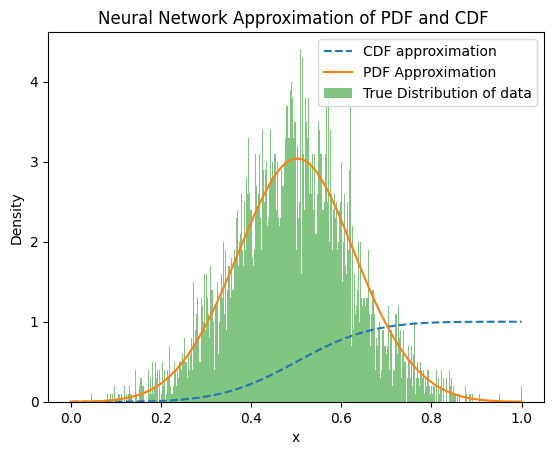
\includegraphics[width=\textwidth]{5ResultsDiscussion/pictures/MarginalTest/NormalHistogram.png}
            %\subcaption*{Histogram}
        \end{minipage}
        \hfill
        \begin{minipage}{0.48\textwidth}
            \centering
            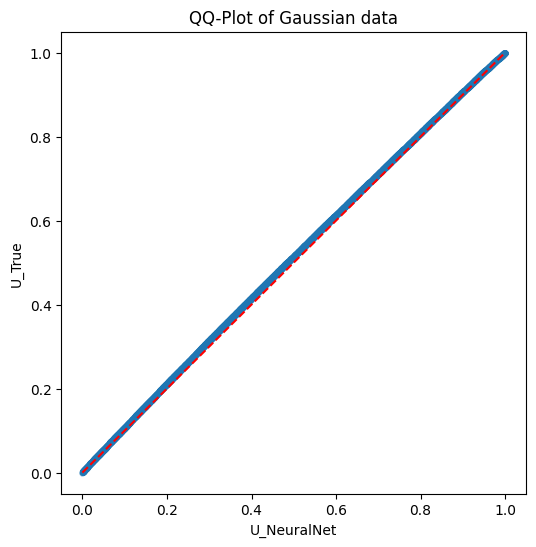
\includegraphics[width=\textwidth]{5ResultsDiscussion/pictures/MarginalTest/NormalQQ.png}
            %\subcaption*{QQ plot}
        \end{minipage}
        \subcaption*{(a) Normal}
    \end{minipage}
    \hfill
    % --- (b) Student's t ---
    \begin{minipage}{0.45\textwidth}
        \centering
        \begin{minipage}{0.48\textwidth}
            \centering
            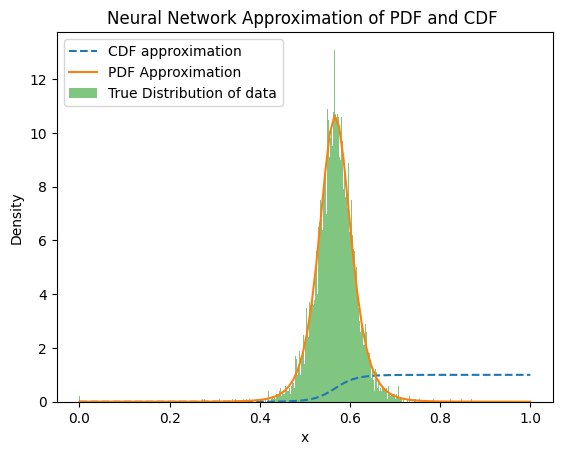
\includegraphics[width=\textwidth]{5ResultsDiscussion/pictures/MarginalTest/StudentsHistogram.png}
            %\subcaption*{Histogram}
        \end{minipage}
        \hfill
        \begin{minipage}{0.48\textwidth}
            \centering
            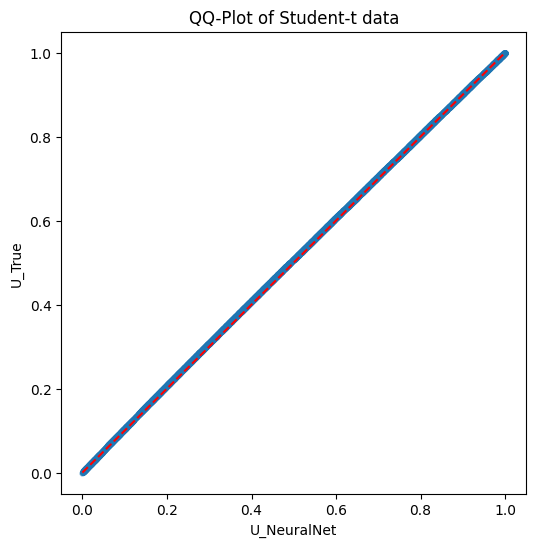
\includegraphics[width=\textwidth]{5ResultsDiscussion/pictures/MarginalTest/StudentsQQ.png}
            %\subcaption*{QQ plot}
        \end{minipage}
        \subcaption*{(b) Student's t}
    \end{minipage}

    \vspace{1em}

    % --- (c) Uniform ---
    \begin{minipage}{0.45\textwidth}
        \centering
        \begin{minipage}{0.48\textwidth}
            \centering
            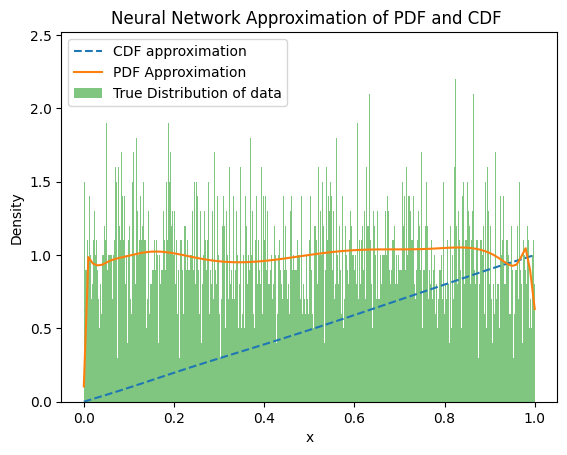
\includegraphics[width=\textwidth]{5ResultsDiscussion/pictures/MarginalTest/UniformHistogram.png}
            %\subcaption*{Histogram}
        \end{minipage}
        \hfill
        \begin{minipage}{0.48\textwidth}
            \centering
            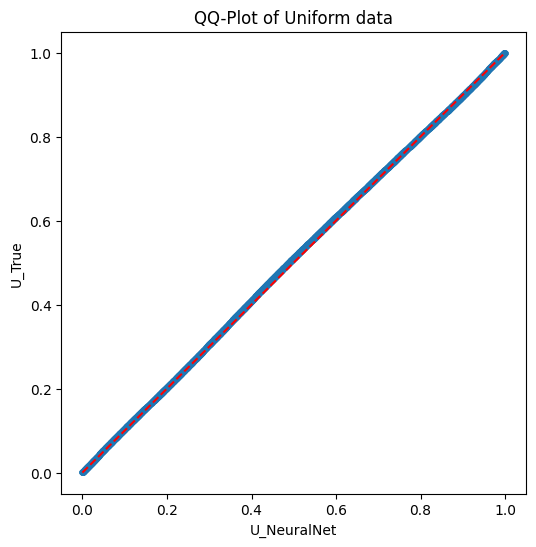
\includegraphics[width=\textwidth]{5ResultsDiscussion/pictures/MarginalTest/UniformQQ.png}
            %\subcaption*{QQ plot}
        \end{minipage}
        \subcaption*{(c) Uniform}
    \end{minipage}
    \hfill
    % --- (d) Exponential ---
    \begin{minipage}{0.45\textwidth}
        \centering
        \begin{minipage}{0.48\textwidth}
            \centering
            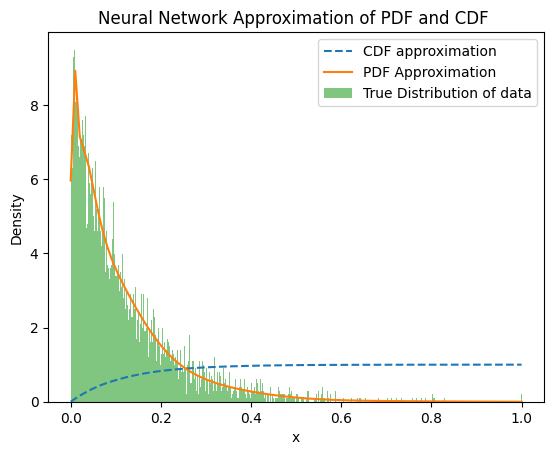
\includegraphics[width=\textwidth]{5ResultsDiscussion/pictures/MarginalTest/ExponentialHistogram.png}
            %\subcaption*{Histogram}
        \end{minipage}
        \hfill
        \begin{minipage}{0.48\textwidth}
            \centering
            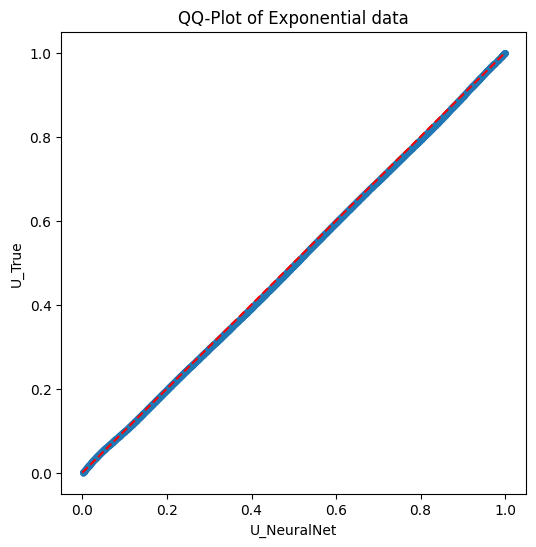
\includegraphics[width=\textwidth]{5ResultsDiscussion/pictures/MarginalTest/ExponentialQQ.png}
            %\subcaption*{QQ plot}
        \end{minipage}
        \subcaption*{(d) Exponential}
    \end{minipage}

    \vspace{1em}

    % --- (e) Laplace ---
    \begin{minipage}{0.45\textwidth}
        \centering
        \begin{minipage}{0.48\textwidth}
            \centering
            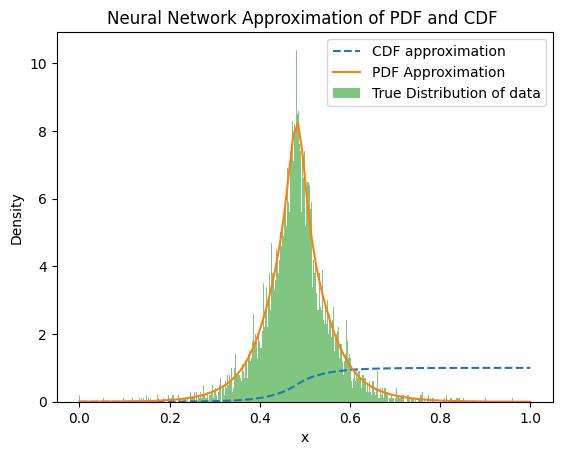
\includegraphics[width=\textwidth]{5ResultsDiscussion/pictures/MarginalTest/LaplaceHistogram.png}
            %\subcaption*{Histogram}
        \end{minipage}
        \hfill
        \begin{minipage}{0.48\textwidth}
            \centering
            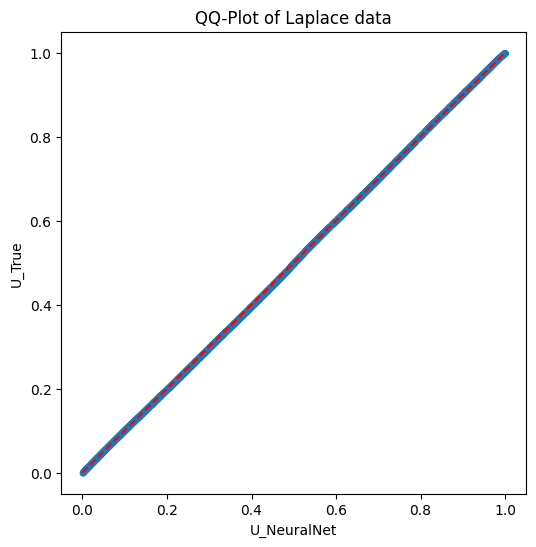
\includegraphics[width=\textwidth]{5ResultsDiscussion/pictures/MarginalTest/LaplaceQQ.png}
            %\subcaption*{QQ plot}
        \end{minipage}
        \subcaption*{(e) Laplace}
    \end{minipage}
    \hfill
    % --- (f) Lognormal ---
    \begin{minipage}{0.45\textwidth}
        \centering
        \begin{minipage}{0.48\textwidth}
            \centering
            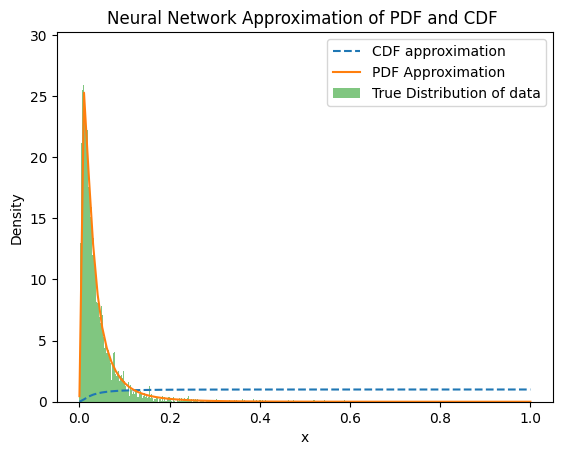
\includegraphics[width=\textwidth]{5ResultsDiscussion/pictures/MarginalTest/LognormalHistogram.png}
            %\subcaption*{Histogram}
        \end{minipage}
        \hfill
        \begin{minipage}{0.48\textwidth}
            \centering
            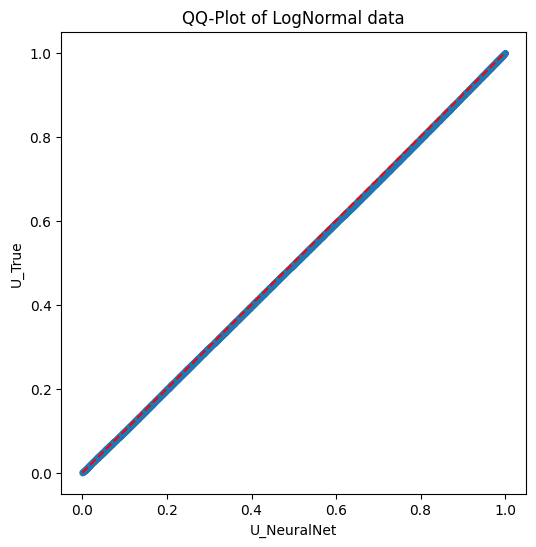
\includegraphics[width=\textwidth]{5ResultsDiscussion/pictures/MarginalTest/LognormalQQ.png}
            %\subcaption*{QQ plot}
        \end{minipage}
        \subcaption*{(f) Lognormal}
    \end{minipage}

    \caption{Marginal distribution visualizations. Each subfigure (a--f) shows a histogram with the trained model and a QQ plot for a distribution.}
    \label{fig:MarginalResults}
\end{figure}


%%%%%%%%%%%%%%%%%%%%%%%%%%%%%%%%%%%%%%%%%%%%%%%%%%%%%%
%% Neural Copula Test   
%%%%%%%%%%%%%%%%%%%%%%%%%%%%%%%%%%%%%%%%%%%%%%%%%%%%%%
\subsection{Neural Copula Test}
The results of the grid search for the hyperparameters and weights are shown in \Cref{tab:Best_hyperparams} and \Cref{tab:Best_weights} respectively. Additionally, the losses for the different datasets using the best hyper parameters and weights are shown in \Cref{tab:LossesBestParameters}. 


\begin{table}[h!]
    \centering
    \caption{The best choice of hyper parameters found in the grid search.}
    \begin{tabular}{ll}
    \textbf{Hyperparameter} & \textbf{Options} \\
    \hline
    Network layers & 3 \\
    Network neurons & 10 \\
    Learning rate & 0.1 \\
    Scheduler & exponential \\
    Solver & Adam \\
    Epochs & 10000 \\
    Batch size & 2014 (Not valid, should remove this as dataset was smaller)\\
    \end{tabular}
    \label{tab:Best_hyperparams}
\end{table}
    
\begin{table}[h!]
    \centering
    \caption{The best choice of weights found for the copula loss function linear combination defined in \Cref{sec:NeuralCopulaLoss}.}
    \begin{tabular}{ll}
    \textbf{Weight} & \textbf{Options} \\
    \hline
    $\lambda_1$ & 1 \\
    $\lambda_2$ & 2 \\
    $\lambda_3$ & 0.5 \\
    $\lambda_4$ & 1 \\
    $\lambda_5$ & 1 \\
    \end{tabular}
    \label{tab:Best_weights}
\end{table}
    

    
\begin{table}[h!]
    \centering
    \caption{Losses for the datasets using the best hyper parameters and weights.}
    % \begin{tabular}{lllllll}
    % \textbf{Dataset} & \textbf{L1}& \textbf{L2}& \textbf{L3}& \textbf{L4}& \textbf{L5}& \textbf{Total Loss} \\
    % \hline
    % Independence & ? & ? & ? &  ? & ? & ?  \\
    % Gaussian, $\rho = 0.7$ & ? & ? & ? &  ? & ? & ? \\
    % Gaussian, $\rho = -0.7$ & ? & ? & ? & ? & ? & ?  \\
    % Upper Frechet Hoeffding bound & ? & ? & ? & ? & ? & ?  \\
    % Lower Frechet Hoeffding bound & ? & ? & ? & ? & ? &   ?  \\
    % \end{tabular}

    \begin{tabular}{lllllll}
        \textbf{Dataset} & \textbf{L1}& \textbf{L2}& \textbf{L3}& \textbf{L4}& \textbf{L5}& \textbf{Total Loss} \\
        \midrule
        Independent & 0.065705 & 0.025223 & 0.045032 & 0.077263 & 0.005574 & 0.218797 \\
        PositiveDependence & 0.290332 & 0.033420 & 0.049284 & 0.239172 & 0.017931 & 0.630140 \\
        NegativeDependence & -0.281669 & 0.025645 & 0.047584 & 0.082656 & 0.005116 & -0.120667 \\
        FrechetUpper & -3.846874 & 0.095704 & 0.257008 & 0.122417 & 0.014359 & -3.357385 \\
        FrechetLower & -3.611439 & 0.080854 & 0.000004 & 0.108494 & 0.003596 & -3.418491 \\
        \end{tabular}
    \label{tab:LossesBestParameters}
\end{table}


\todo{Figure of best fitted copula for the different distributions.}




%%%%%%%%%%%%%%%%%%%%%%%%%%%%%%%%%%%%%%%%%%%%%%%%%%%%%
%% Portfolio Test
%%%%%%%%%%%%%%%%%%%%%%%%%%%%%%%%%%%%%%%%%%%%%%%%%%%%%
\subsection{Portfolio Test}



\begin{table}[h!]
    \centering
    \caption{Distance between the fitted copula and the true distribution for the different distributions. The distance is calculated as described in \Cref{sec:GoodnessOfFit}.}
    \begin{tabular}{lllll}
    \textbf{Dataset/Copula} & \textbf{Gaussian} & \textbf{Students} & \textbf{Clayton} & \textbf{Neural} \\
    \hline
    Gaussian, $\rho$: 0 & ? & ? & ? & ? \\
    Gaussian, $\rho$: 0.7 & ? & ? & ? & ? \\
    Students, $t$ $\rho$: -0.8, df: 3 & ? & ? & ? & ? \\
    Clayton, $\alpha$: 4 & ? & ? & ? & ? \\
    \end{tabular}
    \label{tab:DistributionDistances}
\end{table}

\todo{Figures of the generated data, and fitted copulas.}

\todo{Figure showing copula gradient}


\begin{generalinstructions}
    • Discuss the meaning of your results.\\
    • Discuss the limitations of your results.\\
    • Discuss the relations of your findings to previous knowledge.\\
    • Propose future research direction.\\
\end{generalinstructions}


